As discussed in \autoref{sec:internal-external-nondeterminism}, nondeterminism
makes validators difficult to write.  To address this challenge, I construct
validators {\em automatically} from their specifications.  The key idea is to
encode the specification with a programming language, and {\em dualize} the
specification program into the validator.

This chapter demonstrates the dualization technique with a programming language
in the QAC family.  \autoref{sec:encode-spec} introduces the $\Prog$ language
for encoding specifications.  Specifications written in $\Prog$ are dualized into
validators in \autoref{sec:dualize-prog}, with correctness proven in
\autoref{sec:proof}.

\section{Encoding Specifications}
\label{sec:encode-spec}
Constructing the validator automatically requires analyzing the computations of
the specification program.  The QAC language family in \autoref{sec:qac} only
provides a state monad interface for server models, which is insufficient for
performing structural analysis.  This section introduces a programming language
for encoding specifications.

For readability, I demonstrate the dualization technique on a subset of QAC
server models called integer machine models, featuring random-access memory (RAM)
and arithmetic operations.  To test real-world systems like web servers, I'll
employ a more complex specification language in \autoref{chap:practices}.

\subsection{Integer machine model}
The server state of an integer machine model is a key-value mapping that
resembles a RAM.  The addresses are natural numbers, and the data are integers.
The initial server state has zero data in all addresses:
\begin{align*}
  &s_0:\Nat\to\Int\\
  &s_0=(\_\mapsto0)\\
  &\textit{i.e. }\forall (k:\Nat), s_0!k=0
\end{align*}
Here syntax ``$s!k$'' is pronounced ``data stored in address $!k$ of memory
$s$''.  I use ``$!k$'' to indicate that the natural number $k$ is being thought
of as an address.

The server's query, response, and choices ($Q$, $A$, $C$) are of type integer.
At the beginning of each server loop, the internal choice is written to address
$!0$, and the query is written to address $!1$.  The server then performs some
computation $f:(\Nat\to\Int)\to(\Nat\to\Int)$ that manipulates the memory, and
then sends back the value stored in address $!1$ as the response:
\begin{align*}
  \sstep_f(q,c)(s)\quad\triangleq\quad&\letin{s_1}{\update s0c}\\
  &\letin{s_2}{\update{s_1}1q}\\
  &\letin{s_3}{f(s_2)}\\
  &(s_3!1,s_3)
\end{align*}

Each memory-manipulating computation $f$ defines an instance of the integer
machine model:
\[\existT{S}{\Nat\to\Int}{(\sstep_f,s_0)}\]

Dualizing an integer machine model requires structural analysis of its memory
manipulation.  Next I'll introduce a programming language to encode computations
$(\Nat\to\Int)\to(\Nat\to\Int)$.

\subsection{The $\Prog$ modelling language}
\label{sec:prog-lang}
\paragraph{Syntax}
A program in the $\Prog$ language may read and write at any address of the
memory, perform arithmetic operations, and make conditional branches:
\[\begin{array}{lrll}
\Prog&\triangleq&\Return&\text{end computation}\\
&\mid&!dst\coloneqq\Sexp;\Prog&\text{write to address }dst\in\Nat\\\null
&\mid&\If\Sexp\le\Sexp\Then\Prog\Else\Prog&\text{conditional branch}\\
\Sexp&\triangleq&\Int&\text{constant integer}\\
&\mid&!\src&\text{read from address }\src\in\Nat\\
&\mid&\Sexp\oop\Sexp&op\in\{+,-,\times,\div\}
\end{array}\]

For example, the following program computes the absolute value of data stored in
$!1$, and stores it in address $!1$:
\[\begin{array}{ll}
  \If&!1\le0\\
  \tthen&!1\gets(0-!1);\;\Return\\
  \eelse&\Return
\end{array}\]

\paragraph{Semantics}
Each program $(p:\Prog)$ specifies a computation on the integer machine:
\[\begin{array}{ll}
\multicolumn{2}{l}{\Eval\;:\;\Prog\to(\Nat\to\Int)\to(\Nat\to\Int)}\\
\Eval(p)(s)&\triangleq
\begin{cases}
  s&p\Is\Return\\
  \Eval(p')(\update{s}{\dst}{e^s})&p\Is !\dst\coloneqq e;p'\\
  \Eval(\If {e_1}^s\le{e_2}^s\Then p_1\Else p_2)(s)&p\Is\If e_1\le e_2\Then p_1\Else p_2
\end{cases}\\
e^s&\triangleq
\begin{cases}
  z\hphantom{\Exec(\If {e_1}^s\le{e_2}^s\Then p_1\Else p_2,)}&e\Is z:\Int\\
  s!\src&e\Is !\src\\
  {e_1}^s\oop{e_2}^s&e\Is e_1\oop e_2
\end{cases}
\end{array}\]

Here ``$e^s$'' is pronounced ``evaluating server expression $(e:\Sexp)$ on
memory $(s:\Nat\to\Int)$''.  It substitutes all occurences of ``$!\src$'' with
the data stored in address $!\src$ of memory $s$.

Syntax ``$s[k\mapsto v]$'' is pronounced ``writing value $v$ to address $!k$ of
memory $s$''.  It produces a new memory that maps address $!k$ to $v$, while
other addresses remain unchanged from $s$:
\[s[k\mapsto v]\quad\triangleq\quad k'\mapsto\begin{cases}v&k'=k\\
s!k'&k'\neq k\end{cases}\]

\paragraph{From $\Prog$ to server model}
Every program in the $\Prog$ language corresponds to a server model that
performs the computations it specifies:
\begin{align*}
  &\serverOf:\Prog\to\Server\\
  &\serverOf(p)\;\triangleq\;\existT{S}{\Nat\to\Int}{(\sstep_{\Eval(p)},s_0)}
\end{align*}

For example, the CMP-RST protocol in \autoref{sec:qac-model} can be constructed
by applying $\serverOf$ to the following program:
\[\begin{array}{ll}
\If !1\le!2\Then !1\coloneqq0;\Return&(1)\\
\eelse!1\coloneqq1;!2\coloneqq!0;\Return&(2)
\end{array}\]
The constructed server stores its data $n$ in address $!2$.  When the query
stored in $!1$ is less than or equal to $!2$ (case 1), the server writes $0$ to
address $!1$ as response, and leaves the data untouched in address $!2$.  For
queries greater than $!2$ (case 2), the server writes $1$ as response, and
updates the data in $!2$ with the internal choice stored in $!0$.

Based on specifications written in the $\Prog$ language, we can now construct
the validator automatically by dualization.

\section{Dualizing Specification Programs}
\label{sec:dualize-prog}
This section presents an algorithm that constructs a validator from the
specification program:
\[\validatorOf:\Prog\to\Validator\]

For every program $p$, $\validatorOf(p)$ determines whether a trace is
producible by $\serverOf(p)$:
\begin{align*}
  &\forall (p:\Prog)(t:\List(Q\times A),\\
  &(\behaves{\validatorOf(p)}t)\;\iff\;(\behaves{\serverOf(p)}t)
\end{align*}

More specifically, given a trace of $Q\times A$ pairs, the validator determines
whether there exists a sequences of internal choices $C$ that explains how the
server produces the trace in \autoref{def:trace-validity}.

The idea is similar to the \ilc{tester} in \autoref{sec:interactive-testing},
which \ilc{validate}s the trace by executing the \ilc{serverSpec}, and comparing
the expected response against the tester's observation.

However, executing a nondeterministic specification does not produce a specific
expectation of response, but a space of responses parameterized over the
internal choices.  Therefore, upon observing a response $A$, the validator
should determine whthere there exists a choice $C$ that leads the specification
to produce this response.

This reduces the trace validation problem to constraint solving.  The validator
maintains a set of constraints that unify the responses produced by the
specification against the responses observed from the implementation.

More specifically, the validator executes the $\Prog$ model and represents
internal choices with {\em symbolic variables}.  These variables are carried
along the program execution, so the expected responses are computed as {\em
  symbolic expressions} that might depend on those variables.  The validator
then constrains that the symbolic response is equal to the concrete observation.

To achieve this goal, the validator stores a symbolic variable for each address
of the server model.  It also remembers all the constraints added upon
observation.  This information is called a ``validation state'':
\[(\Nat\to\Var)\times\Set\constraint\]
Here the $\constraint$s are relations between validator expressions ($\Vexp$s)
that may depend on symbolic $\Var$iables:
\[\begin{array}{lrl@{\qquad}l}
\constraint&\triangleq&\Vexp\ccmp\Vexp&cmp\in\{<,\le,=\}\\
\Vexp&\triangleq&\Int&\text{constant integer}\\
&\mid&\#x&\text{variable }x\in\Var\\
&\mid&\Vexp\oop\Vexp&op\in\{+,-,\times,\div\}\\
\end{array}\]
The $\Vexp$ type replaces $\Sexp$'s address constructor $!\src$ with variable
constructor $\#x$.  This allows the validator to constrain the values of the
same address at different times {\it e.g.} the internal choice stored in $!0$ in
different iterations.  The validation state maps each address to its current
representing variable $(\Nat\to\Var)$, which updates as the validator
symbolically executes the server program.

Notice that the server program in \autoref{sec:prog-lang} has conditional
branches.  When executing the specification program, the branch condition might
depend on the internal choices, which is invisible to the validator.  As a
result, the validator doesn't know the exact branch taken by the specification,
so it maintains multiple validation states, one for each possible execution
path:
\[\Set((\Nat\to\Var)\times\Set\constraint)\]

The initial state of the validator is a single validation state that corresponds
to the specification's initial state:
\[\{(\_\mapsto\#0,\{\#0=0\})\}\]
Here the initial validation state says ``all addresses are mapped to variable
$\#0$, and the value of variable $\#0$ is constrained to be zero''.  This
reflects the initial server state that maps all addresses to zero value.

The validator's loop body is derived by dualzing the server model:

\begin{enumerate}
\item \label{rule:write} When the server performs a write operation
  $!\dst\coloneqq \mathit{exp}$, the validator creates a fresh variable $x$ to represent
  the new value stored in address $!\dst$, and adds a constraint that says $x$'s
  value is equal to that of $\mathit{exp}$.  This rule also applies to writing the
  request to address $!1$ before executing the program.
\item \label{rule:branch} When the server makes a nondeterministic branch $\If
  e_1\le e_2\Then p_1\Else p_2$, the validator considers both cases: (a) If
  $p_1$ was taken, then the validator should add a constraint $e_1\le e_2$; or
  (b) If $p_2$ was taken, then the validator should add constraint $e_2<e_1$.
\item \label{rule:choice} Before executing the program, the server writes the internal
    choice $c$ to address $!0$.  Accordingly, the validator creates a fresh
    variable to represent the new value stored in address $!0$, without adding
    any constraint.
\item \label{rule:return} After executing the program, the server sends back the
  value stored in $!1$ as response.  Accordingly, the validator adds a
  constraint that says the variable representing address $!1$ is equal to the
  observed response.
\item \label{rule:unsat} When the constraints of a validation state become
  unsatisfiable, it indicates that the server model cannot explain the
  observation.  This is because either (i) the observation is invalid, i.e.,
  not producible by the server model, or (ii) the observation is valid, but was
  produced by a different execution path of the server model.
\item \label{rule:reject} The validator accepts the trace if it can be produced
  by any execution path of the server model.  Since each execution path
  corresponds to a validation state, the validator only needs to remove the
  unsatisfiable state from the set of states.  If the set of validation states
  becomes empty, it indicates that the observation cannot be explained by any
  execution path of the specification, so the validator should reject the trace.
\end{enumerate}

\begin{figure}
\[\begin{array}{l@{\;}r@{\;}l}
\vstep_p(q,a)(v)&\triangleq&\letin{v'}{v_0\gets v;\vstep'_p(q,a)(v_0)}\\
&&\If v'\Is\varnothing\Then\None\Else\Some v'\hfill(\ref{rule:reject})\\
\vstep'_p(q,a)(v_0)&\triangleq&\letin{v_1}{\Havoc(0,v_0)}\\
&&\letin{v_2}{\Write(1,q,v_1)}\\
&&(\vs_3,\cs_3)\gets\Exec(p,v_2);\\
&&\letin{\cs_4}{\cs_3\cup\{\#(\vs_3!1)= a\}}\hfill(\ref{rule:return})\\
&&\If\solvable \cs_4\Then\{(\vs_3,\cs_4)\}\Else\varnothing\hfill(\ref{rule:unsat})\\
\Exec(p,(\vs,\cs))&\triangleq&\begin{cases}
  \{(\vs,\cs)\}&\text{if }p\Is\Return\\
  \Exec(p',\Write(d,e,(\vs,\cs)))&\text{if }p\Is(!d\coloneqq e;p')\\
  \left(\begin{array}{@{}l}
    \letin{v_1}{(\vs,\cs\cup\{{e_1}^{\vs}\le{e_2}^{\vs}\})}\\
    \letin{v_2}{(\vs,\cs\cup\{{e_2}^{\vs}<{e_1}^{\vs}\})}\\
    \Exec(p_1,v_1)\cup\Exec(p_2,v_2)\hfill(\ref{rule:branch})
  \end{array}\right)&\begin{array}{@{}l@{}l}\text{if }&p\Is\\
    &(\If e_1\le e_2\\
    &\tthen p_1\Else p_2)\end{array}
\end{cases}\\
\Write(d,e,(\vs,\cs))&\triangleq&\letin{x_e}{\Fresh (\vs,\cs)}\hfill(\ref{rule:write})\\
&&(\update{\vs}{d}{x_e},\cs\cup\{\#x_e=e^{\vs}\})\\
\Havoc(d,(\vs,\cs))&\triangleq&\letin{x_c}{\Fresh (\vs,\cs)}(\update{\vs}{d}{x_c},\cs)\hfill(\ref{rule:choice})
\end{array}\]
\caption[Dualizing server model into validator]{Dualizing server model into
  validator, with derivation rules annotated.}
\label{fig:dualize}
\end{figure}

This mechanism is formalized in \autoref{fig:dualize}.  Here the notation
``$v_0\gets v;\vstep'_p(q,a)(v_0)$'' is a monadic bind for sets: Let $\vstep'_p$
map each element $v_0$ in $v$ to a set of validation states
$(\vstep'_p(q,a)(v_0):\Set((\Nat\to\Var)\times\Set\constraint))$, and return the
union of all result sets as $v'$.

The validator adds constraints in three circumstances: \autoref{rule:write} says
the write operation updates the destination with the source expression;
\autoref{rule:branch} guards the branch condition to match its corresponding
execution path; \autoref{rule:return} unifies the server's symbolic response
against the concrete response observed from the implementation.

The constraints added in \autoref{rule:write} and \autoref{rule:branch} are
translated from the specification program.  Given a server expression
$(e:\Sexp)$ from the source expression or the branch condition, syntax $e^\vs$
translates it into a validator expression $\Vexp$ using the validation state
$\vs$, by replacing its addresses with the corresponding variables:
\[e^{\vs}\triangleq\begin{cases}
  n&e\Is z:\Int\\
  \#(\vs!\src)&e\Is!\src\\
  {e_1}^{\vs}\oop{e_2}^{\vs}&e\Is e_1\oop e_2
\end{cases}\]

The validator assumes a constraint solver that can determine whether a set of
constraints is satisfiable, i.e., whether there exists an {\em assignment}
of variables $(\Var\to\Int)$ that satisfies all the constraints:
\begin{gather*}
  \forall \cs,\solvable \cs\iff\exists (\asgn:\Var\to\Int),\satisfy{\asgn}\cs\\
  \begin{array}{r@{\;}l}
    \satisfy{\asgn}\cs\triangleq&\forall(e_1\ccmp e_2)\in \cs, {e_1}^{\asgn}\ccmp{e_2}^{\asgn}\\
    e^{\asgn}\triangleq&\begin{cases}
      z&e\Is z:\Int\\
      \asgn!x&e\Is \#x\\
      {e_1}^{\asgn}\oop{e_2}^{\asgn}&e\Is e_1\oop e_2
    \end{cases}
  \end{array}
\end{gather*}
Here ``$e^{\asgn}$'' is pronounced ``evaluating validator expression $(e:\Vexp)$
with assignment $(\asgn:\Var\to\Int)$''.  It substitutes all occurences of
``$\#x$'' with their assigned value $(\asgn!x)$.

Now we have the algorithm that constructs the validator from the specification
program $p$:
\begin{align*}\validatorOf(p)\;\triangleq\quad&\existT{V}{\Set((\Nat\to\Var)\times\Set\constraint)}\\
  &(\vstep_p,\{(\_\mapsto\#0,\{\#0=0\})\})
\end{align*}

\begin{figure}
\begin{align*}
&\existT{V}{\Set((\Nat\to\Var)\times\Set\constraint)}\\
  &\begin{array}{rll}
     (&\lam{(q,a)(v)}{&\llet v'=\begin{array}[t]{@{}l@{}l@{}ll}
       \multicolumn{3}{@{}l}{(vs_0,cs_0)\gets v;}\\
       \letin{vs_1&}{\update{vs_0}{0}{\Fresh (vs_0,cs_0)}&}&\text{(1)}\\
       \letin{x_q&}{\Fresh (vs_1,cs_0)&}\\
       \letin{vs_2&}{\update{vs_1}{1}{x_q}&}\\
       \letin{cs_2&}{cs_0\cup\{\#x_q= q\}&}\\
       \letin{cs_{3a0}&}{cs_2\cup\{\#(vs_2!1)\le\#(vs_2!2))\}&}&\text{(2a)}\\
       \letin{x_{3a1}&}{\Fresh (vs_2,cs_{3a0})&}\\
       \letin{vs_{3a1}&}{\update{vs_2}{1}{x_{3a1}}&}\\
       \letin{cs_{3a1}&}{cs_{3a0}\cup\{\#x_{3a1}=0\}&}\\
       \letin{cs_{3b0}&}{cs_2\cup\{\#(vs_2!2)<\#(vs_2!1)\}&}&\text{(2b)}\\
       \letin{x_{3b1}&}{\Fresh (vs_2,cs_{3b0})&}\\
       \letin{vs_{3b1}&}{\update{vs_2}{1}{x_{3b1}}&}\\
       \letin{cs_{3b1}&}{cs_{3b0}\cup\{\#x_{3b1}=1\}&}\\
       \letin{x_{3b2}&}{\Fresh (vs_{3b1},cs_{3b1})&}\\
       \letin{vs_{3b2}&}{\update{vs_{3b1}}{2}{x_{3b2}}&}\\
       \letin{cs_{3b2}&}{cs_{3b1}\cup\{\#x_{3b2}=\#(vs_{3b2}!1)\}&}\\
       \multicolumn{3}{@{}l}{((vs_4,cs_4)\gets\{(vs_{3a1},cs_{3a1}),(vs_{3b2},cs_{3b2})\};}&\text{(3)}\\
       \letin{cs_5&}{cs_4\cup\{\#(vs_4!1)= a\}&}\\
       \multicolumn{3}{@{}l}{\If\solvable cs_5\Then\{(vs_4,cs_5)\}\Else\varnothing}\\
       \end{array}\\
       &&\iin\\
       &&\If v'\Is\varnothing\Then\None\Else\Some v'
     }\\
     ,&\multicolumn{2}{l}{\{(\_\mapsto\#0,\{\#0=0\})\}})
   \end{array}
\end{align*}
\caption[Validator for protocol CMP-RST]{Validator for CMP-RST automatically
  derived from its specification in $\Prog$.  This program consists of three
  parts: (1) symbolizing the query and internal choice before executing the
  model, (2) considering both branches in the model program, propagating a
  validation state for each branch, and (3) filtering the validation states by
  constraint satisfiability, removing invalid states.}
\label{fig:derived-validator}
\end{figure}

For example, to construct a validator for the CMP-RST protocol in
\autoref{sec:qac-model}, we first specify it in $\Prog$ as:
\begin{align*}
  &\If!1\le!2\\
  &\tthen!1\gets0;\Return\\
  &\eelse!1\gets0;!2\gets!0;\Return
\end{align*}
This program stores the data $n$ in address $!2$.  If the request is less than
or equal to $n$, then the program writes response $0$ to address $!1$, and
leaves the data unchanged; Otherwise, it writes $1$ as response, and updates
address $!2$ with the internal choice in $!0$.

We then apply function $\validatorOf$ to this $\Prog$-based specification,
resulting in a validator as shown in \autoref{fig:derived-validator}.
Validators constructed in this way are proven correct in the next
section.

\section{Correctness Proof}
\label{sec:proof}
Validators derived in this approach can be proven sound and complete:
\[\begin{array}{r@{\;}l}
\forall p:\Prog,&\letin{s}{\serverOf(p)}\\
&\letin{v}{\validatorOf(p)}\\
&\rejSound v s\wedge\rejComplete v s\\
&\text{\it i.e. }\forall t:\List(Q\times A),\\
&\qquad\valid s t\iff\accepts v t\\
&\qquad\text{\it i.e. }\exists s',\behaves s t s'\iff\exists v',\behaves v t v'
\end{array}\]

In this subsection, I first present a generic framework for proving validators'
correctness properties, and then demonstrate its usage by applying it to
$\Prog$-based validators.

The ``equivalence between server production and validator consumption of all
traces'' is proven by introducing a loop invariant.  The invariant is a
bisimulation between the server and the validator, which is preserved for each
step of the trace produced/consumed.

\subsection{Proving rejection soundness}
The proof of ``any trace produceable by the server is consumable by the
validator'' is by forward induction on the server's execution path.  The
corresponding validation path is constructed based on the following hypotheses:
\begin{itemize}
\item The initial server state reflects the initial validator state:
  \begin{equation}
    \tag{RejSound1}
    \label{eq:rs1}
    \Reflects{(v_0:V)}{(s_0:S)}
  \end{equation}
\item Any server step whose pre-execution state reflects some pre-validation
  state can be consumed by the validator into a post-validation state that
  reflects the post-execution state:
  \begin{align*}
    \tag{RejSound2}
    \label{eq:rs2}
    &\forall(q:Q)(c:C)(a:A)(s,s':S)(v:V),\\
    &\sstep(q,c,s)=(a,s')\wedge\Reflects{v}{s}\\
    &\implies\exists v':V,\vstep(q,a,v)=\Some{v'}\wedge\Reflects{v'}{s'}
  \end{align*}
  \begin{center}
    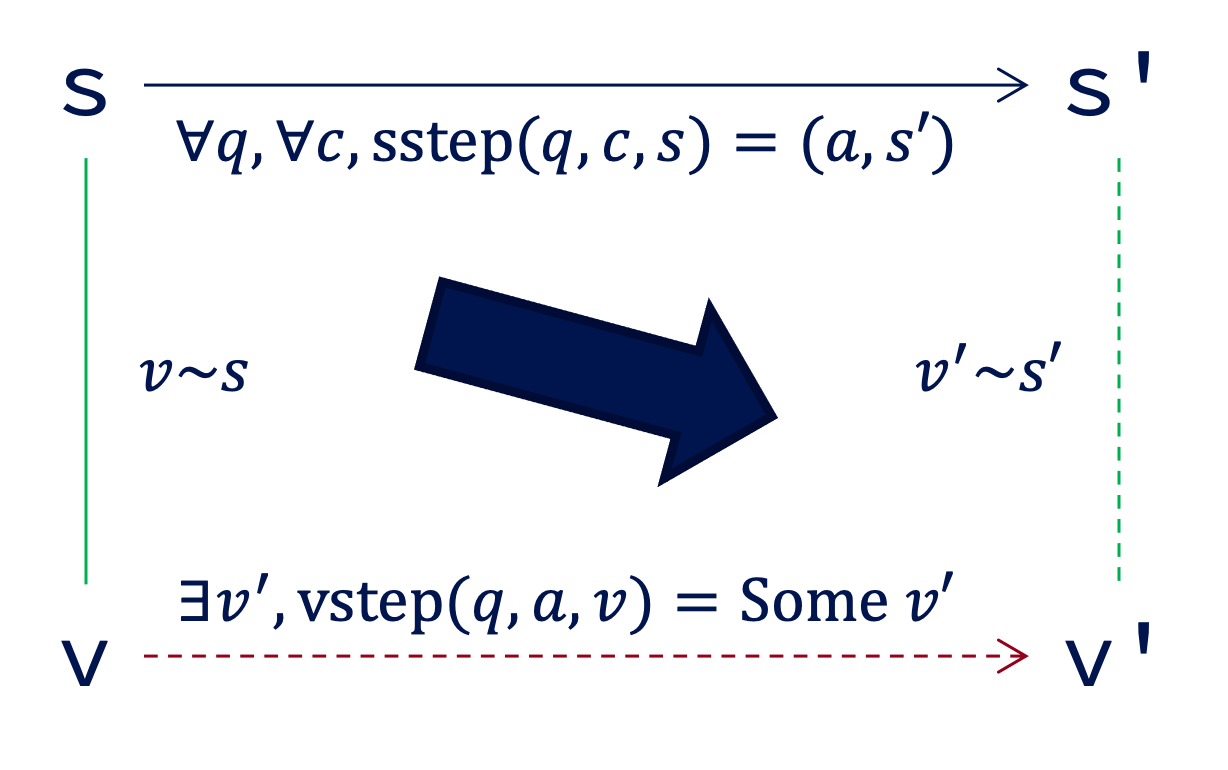
\includegraphics[width=.5\textwidth]{figures/sound}
  \end{center}
\end{itemize}

\subsection{Proving rejection completeness}
The proof of ``any trace consumable by the validator is produceable by
the server'' is by backward induction on the validator's execution
path.  The corresponding server path is constructed based on the
following hypotheses:

\begin{itemize}
\item Any accepting validator step has some server state that reflects the
  post-validation state:
  \begin{align*}
    \tag{RejComplete1}
    \label{eq:rc1}
    \forall(q:Q)(a:A)(v, v':V),\;&\vstep(q,a,v)=\Some{v'}\\
    &\implies\exists s':S,\Reflects{v'}{s'} 
  \end{align*}
\item Any accepting validator step whose post-validation state reflects some
  post-execution server state has a corresponding server step from a
  pre-execution state that reflects the pre-validation state:
  \begin{align*}
    \tag{RejComplete2}
    \label{eq:rc2}
    &\forall(q:Q)(a:A)(v,v':V)(s':S),\\
    &\vstep(q,a,v)=\Some{v'}\wedge\Reflects{v'}{s'}\\
    &\implies\exists(s:S)(c:C),\sstep(q,c,s)=(a,s')\wedge\Reflects{v}{s}
  \end{align*}
  \begin{center}
    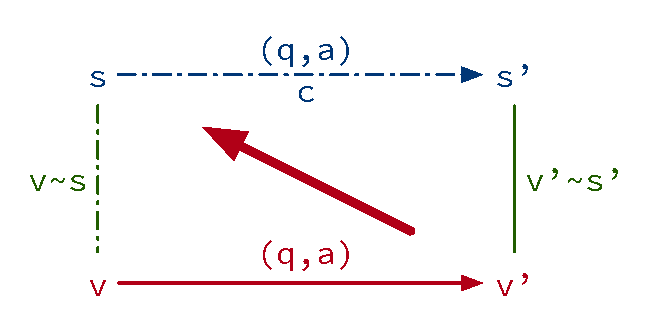
\includegraphics[width=.5\textwidth]{figures/complete}
  \end{center}

\item The initial validator state only reflects the initial server state:
  \begin{equation}
    \tag{RejComplete3}
    \label{eq:rc3}
    \{s\mid\Reflects{v_0}{s}\}=\{s_0\}
  \end{equation}
\end{itemize}

Rejection soundness is proven by forward induction, while rejection completeness
is proven by backward induction.  This is because the choice $c$ is known from
the server step, while unknown from the validator step: Given a validator step,
we cannot predict ``what choices the server will make in the future'', but can
analyze ``what choices the server might have made in the past''.  This proof
method is further explained with the $\Prog$ example:

For specifications written in the $\Prog$ language, the server state is a
mapping from addresses to data; the validation state is a mapping from addresses
to symbolic variables, and constraints over the variables.  A validation state
is accepting if its constraints are satisfiable, {\it i.e.}  there exists an
{\em assignment} of the symbolic variables that can unify the trace with the
server model.  The internal choices made by the server are represented as
symbolic variables.  The assignment maps these variables to the choices' value
at each step, from which we can reconstruct the server's execution path.
\begin{definition}[Bisimulation for $\Prog$ specifications]
  Validator state $v$ {\em simulates} server state $s$ if it contains a
  validation state $(vs,cs)$ that {\em reflects} the server state: (1) There
  exists an assignment $asgn$ that can satisfy the constraints $cs$; and (2) The
  address-variable mapping $vs$ can be {\em instantiated} with the assignment
  (written as ``$vs^{asgn}$'') into an address-data mapping that is equivalent
  with $s$:
  \begin{align*}
    \Reflects v s\quad\triangleq\quad& \exists((vs,cs)\in v)(asgn:\Nat\to\Nat),\satisfy{asgn}
    cs\wedge vs^{asgn}=s\\ vs^{asgn}\quad\triangleq\quad&addr\mapsto
    asgn!(vs!addr)
  \end{align*}
\end{definition}
This bisimulation definition satisfies the hypotheses for proving soundness and
completeness:

Hypotheses~\ref{eq:rs1} and \ref{eq:rc3} are immediate from the initial states'
definition: The initial server state is all-zero map.  The initial validator
state is a singleton that maps all addresses to a variable that is constrained
to have value zero.

\autoref{eq:rc1} is based on the fact that $\vstep_p$ checks the nonemptiness of
the result:
\[\forall q~a~v~v',\vstep_p(q,a,v)=\Some{v'}\implies(\vstep_p'(q,a,v)=v'\wedge\exists (vs,cs)\in v')\]
and that $\vstep_p'$ guards the satisfiability of all constraints in its result:
\[\forall q~a~vs~cs,{(vs,cs)}\in\vstep_p'(q,a,v)\implies\exists asgn,\satisfy{asgn}cs\]

Therefore, any element in the resulting validator state can construct a
simulating server state:
\[\forall asgn~cs~vs~v,(\satisfy{asgn}cs\wedge(vs,cs)\in v)\implies \Reflects{v}{vs^{asgn}}\]

\autoref{eq:rs2} is based on the fact that the pre-validation state must contain
an element that reflects the server's pre-execution state, as defined by the
bisimulation relation.  Given the server's internal choices, we can compute its
execution path.  By induction on the server's execution path, we can construct
the corresponding post-validation state by making the same internal choice and
branch decisions as the server did, and construct the assignment that satisfies
the validator's constraints.

\autoref{eq:rc3} observes that validator design increases the constraints
monotonically.  Therefore, ``assignments that can satisfy the post-validation
constraints'' is a subset of ``assignments that can satisfy the pre-validation
constraints'':
\[\forall q~a~vs~cs~vs'~cs'~asgn,((vs',cs')\in\vstep_p'(q,a,(vs,cs))\wedge\satisfy{asgn} cs')\implies\satisfy{asgn}cs\]

As a result, the corresponding pre-step server state and the internal choice can
be constructed, and proven to perform the server-side step:
\begin{align*}
\forall q~a~vs~cs~vs'~cs'~asgn,\;&(vs',cs')\in\vstep_p'(q,a,(vs,cs))\\
&\implies\sstep_p(q,asgn!(\Fresh{vs}),vs^{asgn})=vs'^{~asgn}
\end{align*}

The intuition here is that the assignment includes ``all choices made by the
server, past and future'', which is narrowed upon more and more observations.
Therefore, the assignment can instantiate all previous validator states into
corresponding servers, and reconstruct the server's execution path by inferring
its internal choices.

